\documentclass[a4paper,14pt]{extreport} 
\usepackage[T2A]{fontenc}
\usepackage[utf8]{inputenc}
\usepackage[english,russian]{babel}
\usepackage{amssymb,amsfonts,amsmath,mathtext,cite,enumerate,float}
\usepackage{graphicx}
\graphicspath{{images/}}
\usepackage{tocvsec2}
\usepackage{setspace}
\usepackage[normalem]{ulem}


\usepackage{geometry} 
\geometry{left=3cm}
\geometry{right=1.5cm}
\geometry{top=2cm}
\geometry{bottom=2cm}

\renewcommand\thesection{\arabic{section}}
\renewcommand\thechapter{\arabic{chapter}}

\renewcommand{\baselinestretch}{1.5}

\begin{document}
\begin{titlepage}
\newpage
 \begin{center}
  
    Министерство образования Республики Беларусь\\
    \vspace{1em}
    Учреждение образования\\
  \textsc{Белорусский государственный университет информатики и радиоэлектроники}
    \vspace{2em}
    \begin{flushleft}
    Факультет компьютерных систем и сетей\\
	 \vspace{1em}
    Кафедра программного обеспечения информационных технологий\\
	 \vspace{1em}
   Дисциплина: Компьютерные системы и сети\\
	 \vspace{1em}
    \end{flushleft}
    
	\vspace{5em}
    \textsc{Пояснительная записка}\\ к курсовому проекту\\на тему\\
    \bigskip
    {Сайт-журнал}\\
      \bigskip  
    БГУИР КП  I-40 01 01  312  ПЗ
  
\end{center}

\vspace{8em}

\begin{flushleft}
	
	Выполнил:\\
	студент гр.351003 \hspace{7cm} Левошко Н.А.\\ 
	Проверил: \hspace{8.6cm} Третьяков Ф.И.
\end{flushleft}

\vfill


\begin{center}
   Минск, 2015
\end{center}
\end{titlepage}
\center
Задание\\
по курсовому проектированию\\
\medskip
\endcenter
\raggedright
Студенту \underline{Левошко Николаю Андреевичу}\\

\item Тема работы \underline{Веб-приложение сайт-журнал}\\ 
\item Срок сдачи \underline{09.06.2015}
\item Исходные данные \underline{документы формата .tpl, .php и .html}

\item Содержание записки (перечень вопросов, которые подлежат разработке)\\
\underline{\hspace*{16cm}}\hspace*{-16cm}Введение. 1. Анализ прототиповб литературных источников и\\ \underline{\hspace*{16cm}}\hspace*{-16cm}формирование требований к проектироемому приложению. 2. Анализ\\
\underline{\hspace*{16cm}}\hspace*{-16cm} требований к приложению и разработка функциональных требований.\\
\underline{\hspace*{16cm}}\hspace*{-16cm} 3.Проектирование, создание(конструирование) приложения.\\
\underline{\hspace*{16cm}}\hspace*{-16cm} 4. Тестированиеб проверка работоспособности и анализ полученных\\
\underline{\hspace*{16cm}}\hspace*{-16cm} результатов. 5.Руководство по установке и использованию приложения.\\
\underline{\hspace*{16cm}}\hspace*{-16cm} Заключение. Список использованной литературы. Приложения.
\item Перечень графического материала (с точным обозначением обязательных чертежей и графиков)\\
\item Консультант по курсовой работе\\
\underline{Третьяков Ф.И.} 
\item Дата выдачи задания \underline{DD.MM.YYYY}
\item Календарный график работы над проектом на весь период проектирования (с обозначением сроков выполнения и процентом от общего объёма работы):\\
\underline{\hspace*{16cm}}\hspace*{-16cm}раздел 1 к DD.MM.YYYY – 15 \% готовности работы;\\ 
\underline{\hspace*{16cm}}\hspace*{-16cm}разделы 2, 3 к DD.MM.YYYY – 30 \% готовности работы;\\ 
\underline{\hspace*{16cm}}\hspace*{-16cm}раздел 4 к DD.MM.YYYY – 60 \% готовности работы;\\
\underline{\hspace*{16cm}}\hspace*{-16cm}раздел 5, 6 к DD.MM.YYYY – 90 \% готовности работы;\\
\underline{\hspace*{16cm}}\hspace*{-16cm}оформление пояснительной записки и графического материала к\\
\underline{\hspace*{16cm}}\hspace*{-16cm}DD.MM.YYYY – 100 \% готовности работы.\\
\underline{\hspace*{16cm}}\hspace*{-16cm}Защита курсового проекта с DD по DD июля YYYY г.\\

\hspace*{7cm}РУКОВОДИТЕЛЬ\underline{\hspace*{4cm}}\hspace*{-3.9cm}Третьяков Ф.И.\\
\hspace*{11.5cm}\small (подпись) \normalsize\\
\bigskip
Задание принял к исполнению \underline{\hspace*{10.5cm}}\hspace*{-8cm}Левошко Николай Андреевич 09.06.2015г.\\
\hspace*{7cm}\small (дата и подпись студента) \normalsize\\

\newpage
\renewcommand\contentsname{\normalsize СОДЕРЖАНИЕ}
\tableofcontents 

\parindent=1.25cm
\newpage

\section*{\normalsize ВВЕДЕНИЕ}
\addcontentsline{toc}{section}{ВВЕДЕНИЕ}

\label{sec:intro}
	\hspace{4ex}В современном мире высоко развиты сферы оказания услуг. Повсеместно можно увидеть предложения о оказании услуг в любой области.
	И интернет, как очень распространнёная и большая часть информационного пространства, может помочь людям как найти предложения о услугах, так и опубликовать их. Самым широкоиспользуемым и применяемым методом являются различные веб-		сайты.\\
	\hspace{4ex} С каждым днем численность интернет-аудитории растёт, тем самым расширяя возможности поиска потенциальных клиентов. Все большее число людей прибегают к поиску необходимых товаров и услуг в сети, и если Ваша продукция в 		отличие от конкурентов не представлена в интернете, Вы можете потерять значительную часть рынка.\\
	\hspace{4ex}Интернет во многом решил проблему коммуникации между отдаленными регионами. Имея собственный сайт, Вы можете с легкостью заявить о себе не только местным жителям, но и тем, кто проживает за тысячи километров от Вашего 		местонахождения.\\
	\hspace{4ex} Большинство людей предпочитают пользоваться услугами или покупать товары тех фирм, которые открыто рассказывают о своей деятельности. Веб-сайт – отличный способ продемонстрировать открытость и создать имидж надежной и 		серьезной компании.\\
	\hspace{4ex}Технологии современного веб-сайта позволяют создавать удобную систему обратной связи, которая помогает изучить мнения клиентов, выявить слабые места и оперативно среагировать на изменения на рынке. Кроме того, возможность 		доступной связи с производителем позволяет повысить лояльность к бренду.\\
	\hspace{4ex}Благодаря развитию методов разработки веб-сайтов, сейчас на Интернет-страничках можно размещать не только текстовое и графическое описание услуг и товаров, но и публиковать видео-материалы, которые максимально полно 			продемонстрируют все преимущества предлагаемой продукции.\\
	\hspace{4ex}Интернет-сайт не требует присутствия на рабочем месте. И все желающие могут получить необходимую информацию о компании или заказать продукцию в любой момент времени.\\
	\hspace{4ex}Знакомство с продукцией на веб-сайте в отличие от надоевшей рекламы по радио и ТВ может быть гораздо эффективнее, поскольку так потенциальные клиенты будут получать интересующую их информацию (о Ваших товарах и услугах) 		по собственной воле.\\
	\hspace{4ex}На веб-сайте можно опубликовать всю возможную информацию о компании и продукции, контакты, схемы проезда, цены и прочее. Таким образом Вы избежите большого числа звонков и направите освободившееся время на развитие 			компании.\\
	\hspace{4ex}Представительский веб-сайт - еще один способ поиска и установления новых партнерских связей, которые дают немало возможностей для развития. При этом сфера поиска не будет ограничена географией.
	Нам повезло жить в эпоху развития информационных технологий и Интернета в частности. Всемирная сеть предлагает неисчерпаемые возможности для развития бизнеса любой сферы деятельности. Но в качестве основы всегда должен быть хороший 		веб-сайт, отвечающий целям и принципам организации и имеющий высокий показатель конверсии. \\

\newpage
\section{\normalsize АНАЛИЗ ПРОТОТИПОВ, ЛИТЕРАТУРНЫХ ИСТОЧНИКОВ И ФОРМИРОВАНИЕ ТРЕБОВАНИЙ К ПРОЕКТИРУЕМОМУ ППРИЛОЖЕНИЮ}
\label{sec:exp}


\subsection{\normalsize Анализ литературных источников}
\label{sec:exp:analog}
\hspace{1.25cm} Сайт (от англ. website: web — «паутина, сеть» и site — «место», буквально «место, сегмент, часть в сети») — система электронных документов (файлов данных и кода) частного лица или организации в компьютерной сети под общим адресом (доменным именем или IP-адресом).
Все сайты в совокупности составляют Всемирную паутину, где коммуникация (паутина) объединяет сегменты информации мирового сообщества в единое целое — базу данных и коммуникации планетарного масштаба. Для прямого доступа клиентов к сайтам на серверах был специально разработан протокол HTTP.
	Браузер —прикладное программное обеспечение для просмотра веб-страниц; содержания веб-документов, компьютерных файлов и их каталогов; управления веб-приложениями; а также для решения других задач. В глобальной сети браузеры используют для запроса, обработки, манипулирования и отображения содержания веб-сайтов. Многие современные браузеры также могут использоваться для обмена файлами с серверами ftp, а также для непосредственного просмотра содержания файлов многих графических форматов (gif, jpeg, png, svg), аудио-видео форматов (mp3, mpeg), текстовых форматов (pdf, djvu) и других файлов.
	Всемирная паутина  — распределённая система, предоставляющая доступ к связанным между собой документам, расположенным на различных компьютерах, подключенных к Интернету. Для обозначения Всемирной паутины также используют слово веб (англ. web «паутина») и аббревиатуру WWW. Всемирную паутину образуют сотни миллионов веб-серверов. Большинство ресурсов всемирной паутины основаны на технологии гипертекста. Гипертекстовые документы, размещаемые во Всемирной паутине, называются веб-стран	ицами. Несколько веб-страниц, объединённых общей темой, дизайном, а также связанных между собой ссылками и обычно находящихся на одном и том же веб-сервере, называются веб-сайтом. Для загрузки и просмотра веб-страниц используются специальные программы — браузеры (англ. browser)
 Разработанное веб-приложения предназначается для размещения информации о предоставляемых услугах, а так же размещения тематических статей.
Разработаны функции для отображения вышеперечисленной информации.
Веб-приложение не требует каких-либо входных данных. Обращение происходит путём ввода адреса сайта в адресную строку браузера.
Выходными данными являются html-страницы, которые преобразуются браузером в удобный для чтения пользователю вид.
Временные характеристики ограничиваются скоростью интернет соединения пользователя.
Надёжность веб-приложения находится на высоком уровне, так как пользователь не может вносить какие-либо данные или как-либо влиять на работу сайта.
Для разработки данного веб-приложения был выбран язык программирования php, так как он хорошо подходит для разработки шаблонизаторов. Также был выбран язык разметки HTML5, так как он широко используется для разработки веб-страница сайтов.

\subsection{\normalsize Анализ прототипов и программ аналогов}
\label{sec:exp:analog}
\hspace{1.25cm}Cайт texnoxors.ru — Сайт посвящён поставке подшипников, запорной арматуры, газового и теплоэнергетического оборудования. ТехноХОРС осуществляет поставки промышленной трубопроводной арматуры, применяемой в тепловой и атомной энергетике, химической, нефтяной, газовой и других отраслях промышленности. Сайт выполнен в стиле "визитки" с описание товара и контактной информацией.
	\center{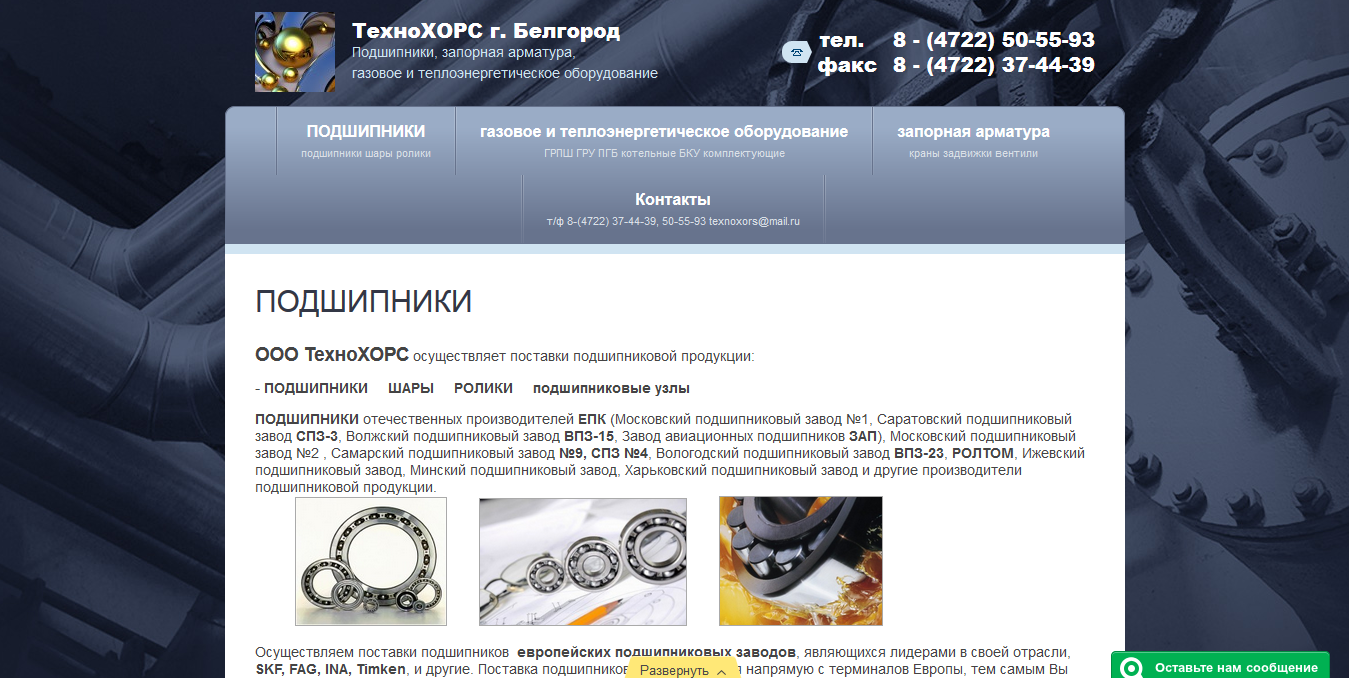
\includegraphics[width=0.7\linewidth]{analog1}}\\
	Сайт bkonsultant71.ru – Это сайт посвящён бухгалтерским услугам в Туле, оказываемых организациям и индивидуальным предпринимателям. Этот сайт, так же как и предыдущий выполнен в виде "визитки". На главной странице 
	отображён перечь оказываемых услуг и цены на них, а так же контактные данные.
	\center{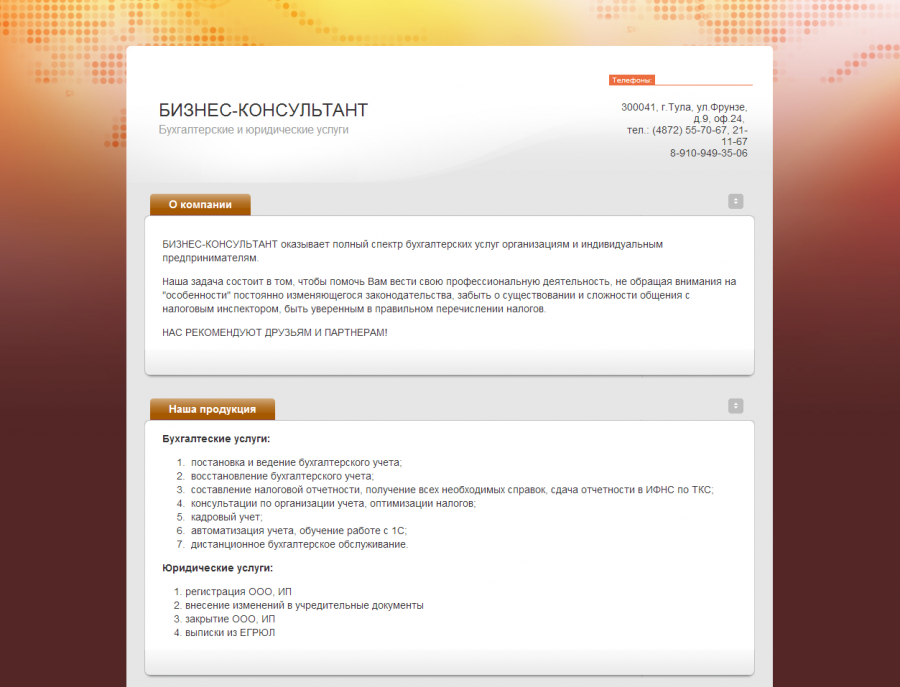
\includegraphics[width=0.7\linewidth]{analog2}}

\subsection{\normalsize Формирование требований к разрабатываемому приложению}
\label{sec:exp:analog}
\hspace{1.25cm}На основе проведенного анализа требования к проектируемому программному средству являются следующими:

а)	программа должна осуществлять отображение информации об оказываемых услугах;

б)	программа должна осуществлять изображение информации о контактах;

в)	программа должна осуществлять  размещение тематических статей.

г)	программа должна предусматривать переход по страницам сайта.

д)	предоставлять функцию доработки содержимого сайтаl.

Данная программа предназначена для личного использования.  

Веб-приложение «Сайт-журнал» должно иметь ряд функций и процедур, организованных для выполнения поставленной задачи. Структура и описание таких функций и процедур будет подробно описано в последующих разделах.

Для реализации данной курсовой работы был выбран язык программирования PHP, позволяющий реализовать архитектуру приложения, а также язык разметки HTML5 и каскадная таблица стилей CSS3.

 Данное приложение обладает удобным и понятным интерфейсом, который не требует каких-либо знаний программирования у пользователя и знаний в сфере информационных технологий в целом. То есть этой программой сможет воспользоваться любой пользователь, когда-либо работавший на компьютере. 
 
 Приложение требует минимальное количество оперативной памяти, занимает минимум места на жестком диске. Требует наличия любого браузера, а также настроенного локального сервера Apache. Однако требуется наличие подключения к сети интернет.

\newpage
\section{\normalsize АНАЛИЗ ТРЕБОВАНИЙ К ПРИЛОЖЕНИЮ И РАЗРАБОТКА ФУНКЦИОНАЛЬНЫХ ТРЕБОВАНИЙ}

\subsection{\normalsize Описание функциональности приложения}
\label{sec:exp:analog}
\hspace{1.25cm} Для удобства доработки данного веб-приложения, был создан шаблонизатор на языке php.
Концепция шаблонизатора состоит в том, чтобы разделять логику получения данных от логики отображения данных
 Шаблонизатор— программное обеспечение, позволяющее использовать html-шаблоны для генерации конечных html-страниц. Основная цель использования шаблонизаторов — это отделение представления данных от исполняемого кода. 		Часто это необходимо для обеспечения возможности параллельной работы программиста и дизайнера-верстальщика. Использование шаблонизаторов часто улучшает читаемость кода и внесение изменений во внешний вид, когда проект целиком 	выполняет один человек.
Сайт был разработан  в минималистичном стиле, однако он содержит всю необходимую информацию о предостовляемых услугах. Таким образон реализованы следующие пункты:
\begin{itemize}
	\item Сайт не требует пристального внимания, обслуживания и постоянного обновления контента.
	\item Достаточно простой сайт, предоставляет только самую важную информацию.
	\item Возможно модернизировать сайт в будущем
\end{itemize}
Данное веб-приложение содержит информацию о контактах, разнообразные тематические статьи, информацию об оказываемых услугах, а также стоимость этих услуг.
Всё это отображается в виде слайдера, а так же в виде текста с изображениями на страницах сайта.
Пользователь,  после отправки запроса на сайт, сможет увидеть главную страницу сайта, и затем перейти на нужную страницу.

\subsection{\normalsize Спецификация  функциональных требований}
\label{sec:exp:analog}
\hspace{1.25cm}1.	Пользователю должен быть предоставлен выбор, на какую страницу сделать переход.
2.	Пользователь должен иметь возможность получить информацию об оказываемых услугах.

3.	Пользователь должен иметь возможность получить информацию о контактах.

4.	Пользователь должен иметь возможность чтения рализчных тематических статей.


\newpage
\section{\normalsize ПРОЕКТИРОВАНИЕ, СОЗДАНИЕ (КОНСТРУИРОВАНИЕ) ПРИЛОЖЕНИЯ}
\label{sec:pc}
\subsection{\normalsize Описание используемых алгоритмов}
\label{sec:exp:pc}
\begin{center}
\textbf{Шаблонизатор} 
\end{center}
Концепция шаблонизатора состоит в том, чтобы разделять логику получения данных от логики отображения данных.

Шаблонизатор находит при помощи регулярных выражений и  записывает в массив строк, содержащий название tpl файлов, в файле страницы, затем извлекает содержимое этих файлов и подставляет их в готовую для вывода веб-страницу.
	Шаблонизатор реализован при помощи двух методов, таких как  getplaceholders, который находит названия tpl файлов и записывает их в массив и output, который распологает содержимое этих файлов в структуру страницы.
В файлах самих страниц, на который поступает запрос содержится лишь подключение шаблонизатора, создание экземпляра класса и вывод содержимого готовой страницы.
Реализация шаблонизатора:
\begin{verbatim}
<?php
class Template
{
	private $file;
	
	public function __construct($file)
	{
		$this->file = $file;
	}
	
	public function output()
	{

		$output = file_get_contents($this->file);
			$changed = true;
			while ($changed)
			{
				$changed = false;
				$placeholders = $this->get_placeholders();
				foreach ($placeholders as $key => $value)
				{
					$tag_to_replace = $value;
					$output_copy = $output;
					$template_name = 'templates/' . str_replace("{include(\"", "", $value);
					$template_name = str_replace("\")}", "", $template_name) . '.tpl';
					$output = str_replace($tag_to_replace, file_get_contents($template_name), $output);
					if ($output !== $output_copy)
					{
						$changed = true;
					}
				}
			}		
		return $output;
	}
	
	private function get_placeholders()
	{
		$template = file_get_contents($this->file);
		$pattern = '/{include\(.+?\)}/';
		
		$matches = array();
		preg_match_all($pattern, $template, $matches);
	
		return $matches[0];
	}

	
}	
\end{verbatim}	

Сами tpl файлы содержат html-код, при помощи которого конструируется будущий вид страницы.
В файлах страниц содержить подключение таблицы стилей, для более удобного и красочного отображения страницы, а так же файлы javascript, в которых реализован слайдер, используемый на двух страницах сайта, был использован слайдер easyslider.
Структура сайта состоит из заголовка, плавающего меню, блока с информационной частью.
В заголовке находится название страницы и ссылка на главную страницу сайта.
В плавающем меню расположены ссылки на остальные страницы сайта.
В информационном блоке содержится информация, зависящая от открытой пользователем страницы.
Реализация одного tpl файла:
\begin{verbatim}
	
			<div id="menu">
			<ul>
			<li><a class="links" href="contacts.php">Контакты</a></li>
			<li><a class="links" href="price.php">Услуги и цены</a></li>
			<li><a class="links" href="topics.php">Статьи</a></li>
			</ul>
			</div>
				<div id="content">
		
					<div id="container">

						<div id="sliderheader">
							<h1>Качественная проводка</h1>
						</div>
							<div id="slidercontent">
								<div id="slider">
									<ul>				
										<li><a href=""><img src="images/03.jpg" alt="Css Template Preview" /></a></li>
										<li><a href=""><img src="images/04.jpg" alt="Css Template Preview" /></a></li>
										<li><a href=""><img src="images/03.jpg" alt="Css Template Preview" /></a></li>
										<li><a href=""><img src="images/04.jpg" alt="Css Template Preview" /></a></li>
										<li><a href=""><img src="images/05.jpg" alt="Css Template Preview" /></a></li>			
									</ul>
								</div>
							</div>

					</div>

				</div>
\end{verbatim}
Реализация файла страницы:
\begin{verbatim}
<?php
include("template.php");
$template = new Template("templates/page-template.html");
echo $template->output();
\end{verbatim}

\newpage
\section{ \normalsize ТЕСТИРОВАНИЕ, ПРОВЕРКА РАБОТОСПОСОБНОСТИ И АНАЛИЗ ПОЛУЧЕННЫХ РЕЗУЛЬТАТОВ}
\label{sec:test}
\subsection{\normalsize Проверка работоспособности}
\hspace{1.25cm}
На изображениях ниже приведены доказательства корректной   работы веб-приложения.
\center{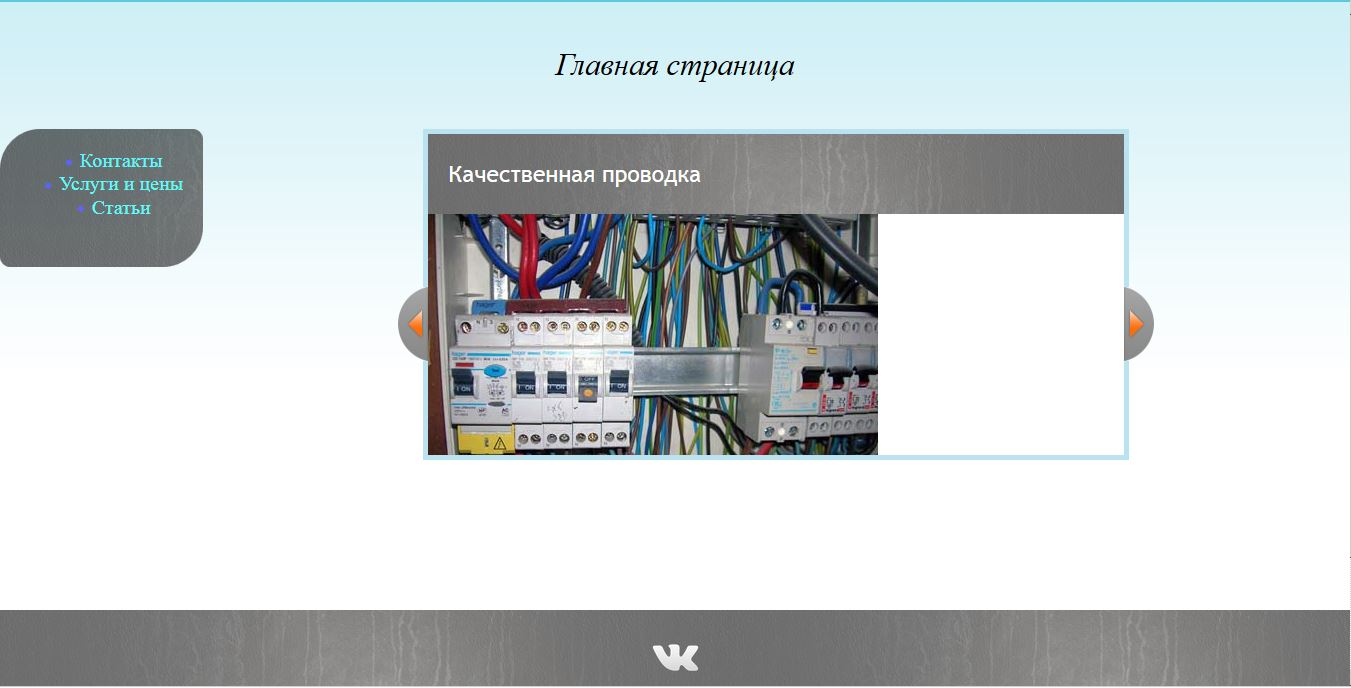
\includegraphics[width=0.7\linewidth]{mainpage}}\\
Рис.1 Работа главной страницы сайта.
Изображено меню со ссылками на другие страницы, слайдер и информационные элементы страницы.

\center{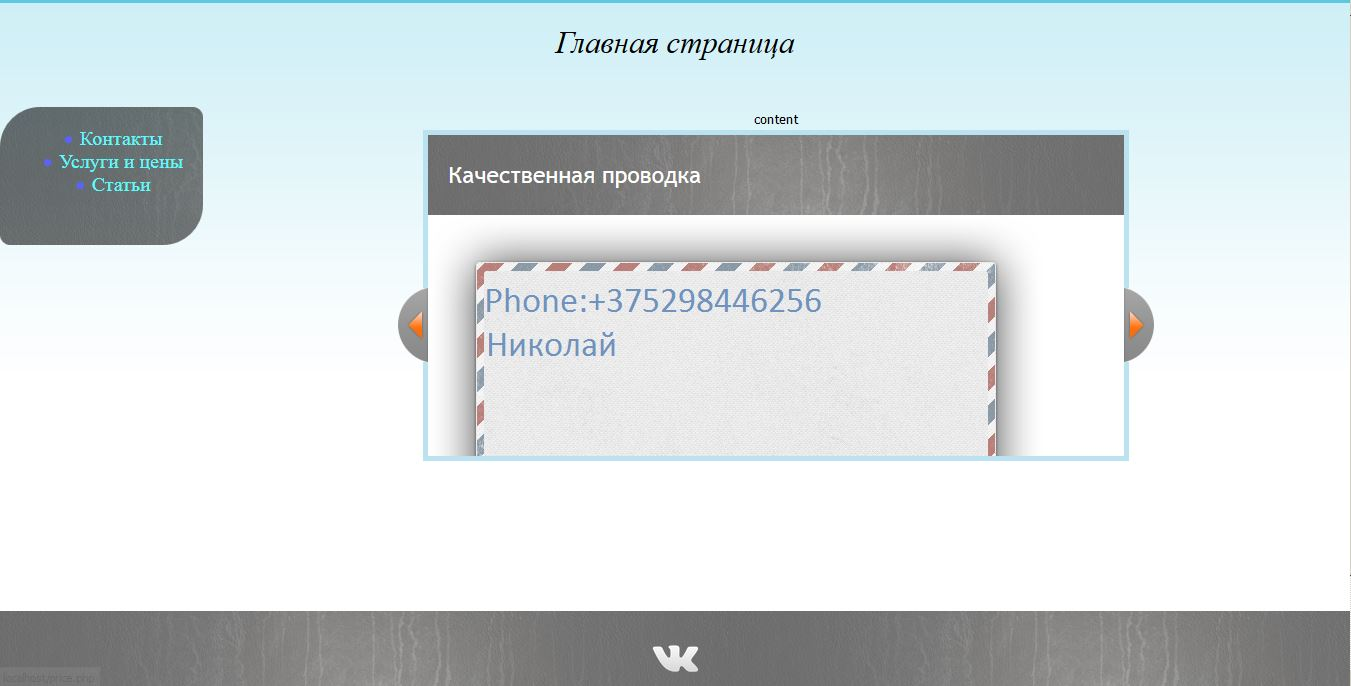
\includegraphics[width=0.7\linewidth]{contactpage}}\\
Рис.2 Работа контактной страницы сайта.
Изображено меню со ссылками на другие страницы, слайдер и контактный данные.

\center{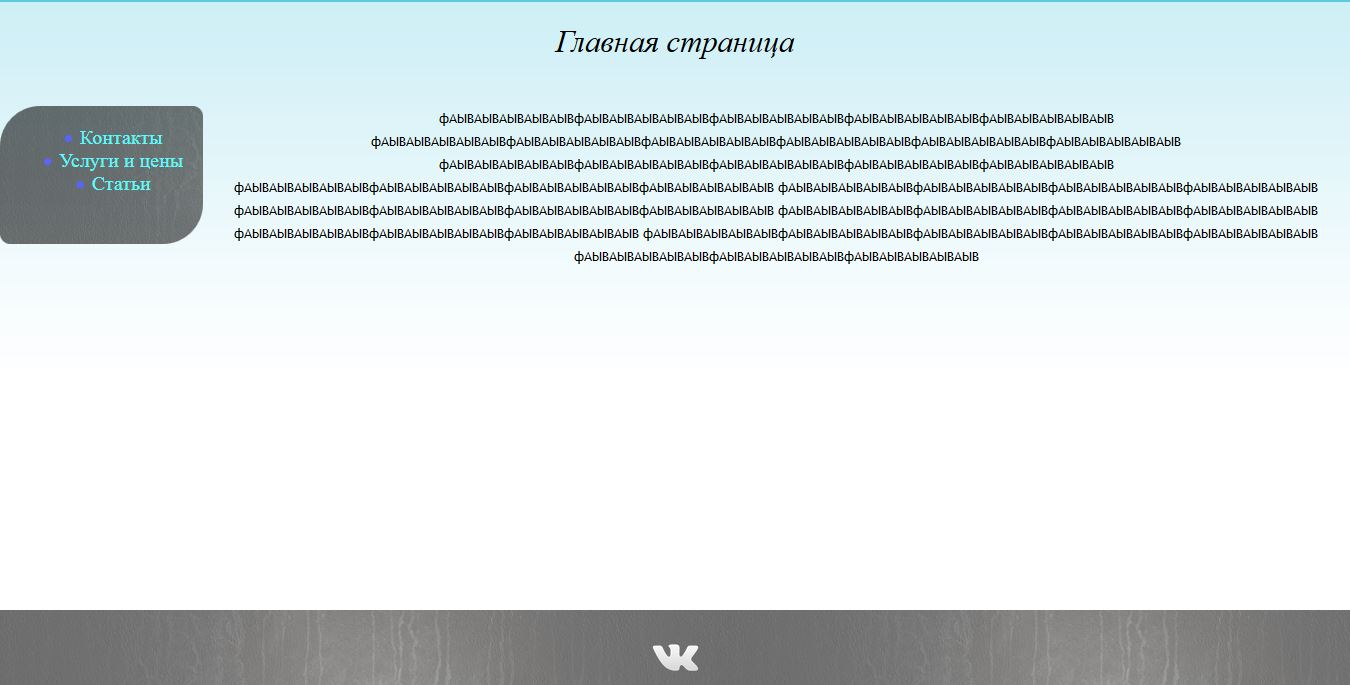
\includegraphics[width=0.7\linewidth]{pricepage}}\\
Рис.3 Работа страницы сайта, содержащий услуги и цены.
Изображено меню со ссылками на другие страницы, предостовляемые услуги и их стоимость.


\center{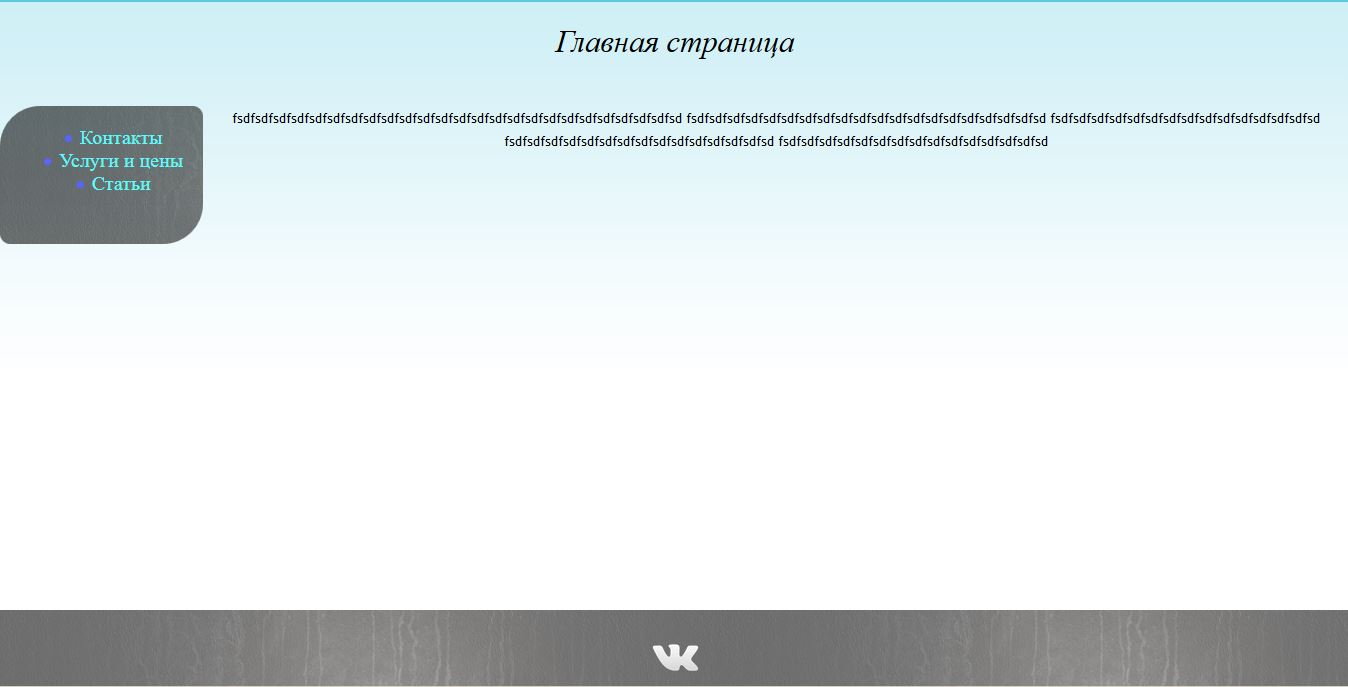
\includegraphics[width=0.7\linewidth]{topicspage}}\\
Рис.4  Работа страницы сайта, содержащей статьи.
Изображено меню со ссылками на другие страницы, тематические статьи.
\subsection{\normalsize Тестирование}
\hspace{1.25cm}


\newpage
\section{\normalsize РУКОВОДСТВО ПО УСТАНОВКЕ И ИСПОЛЬЗОВАНИЮ ПРИЛОЖЕНИЯ}
\hspace{1.25cm}Прежде чем запускать приложение необходимо настроить локальный сервер Apache. Подробную инструкцию по установке и настройке Apache вы можете увидить здесь: 
http://www.webbcare.org/lectures/web-servers/Lecture15.pdf.

Можно также воспользовать уже настроенными пакетами, такими как xampp (https://www.apachefriends.org/ru/index.html) или denver \\
(http://www.denwer.ru/). 
Файлы, при распаковке, следует поместить в папку htdocs (все скрипты, запускаемые на локальной машине
по умолчанию, находятся в данной папке) в уже настроеном Apache.
\center{\includegraphics[width=0.7\linewidth]{setup}}\\
Далее запускаем браузер. В адресной строке необходимо прописать путь к файлу: http://localhost/htdocs/(название страницы, либо оставить пустым).
Приложение готово к использованию.\\
Так же можно воспользоваться установочным файлом SetupWebsite.exe
Файл был создан при помощи программы Smart Install Maker
После запуска программы необходимо следовать инструкция установки.
\center{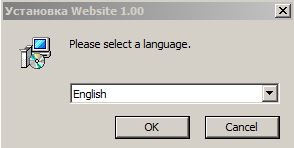
\includegraphics[width=0.7\linewidth]{setuper1}}\\
Первый  шаг установки- выбор языка установки.

\center{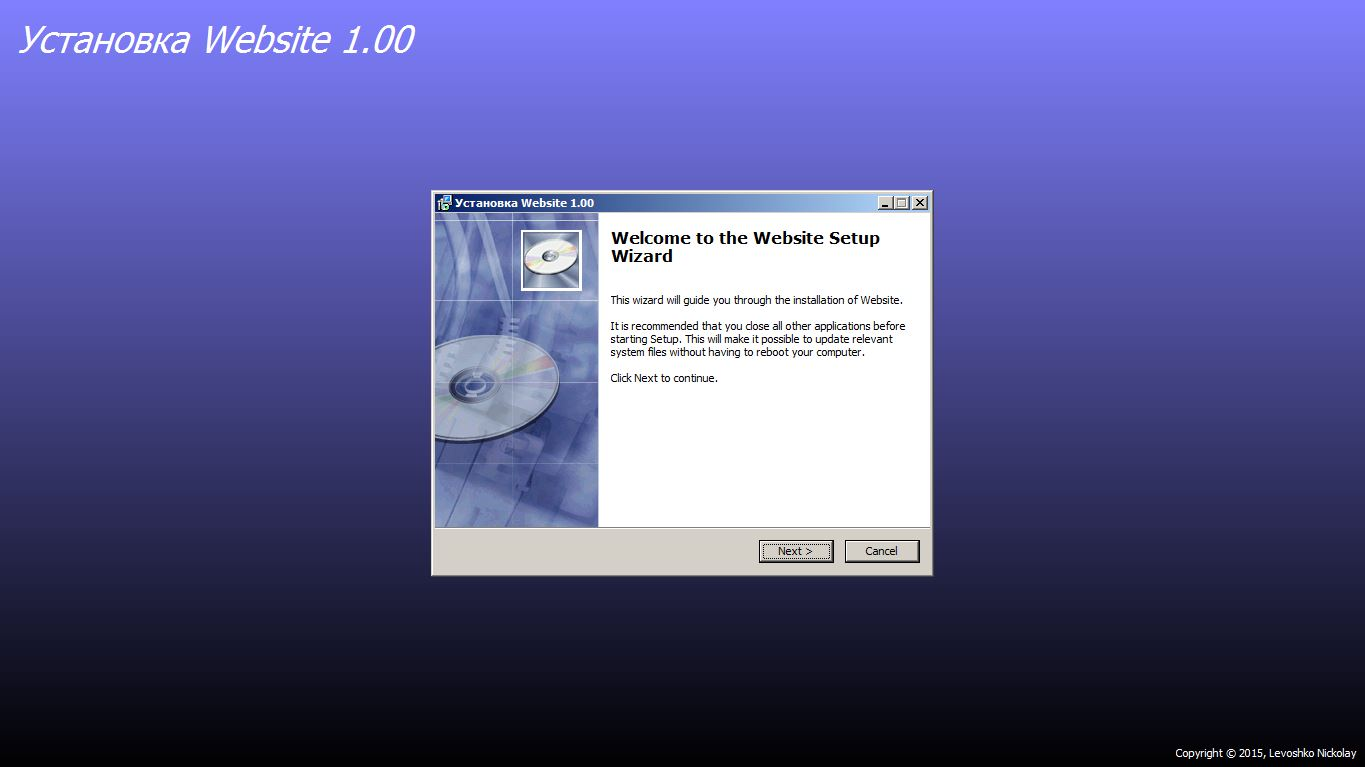
\includegraphics[width=0.7\linewidth]{setuper2}}\\
Второй шаг установки- подтверждение.
\center{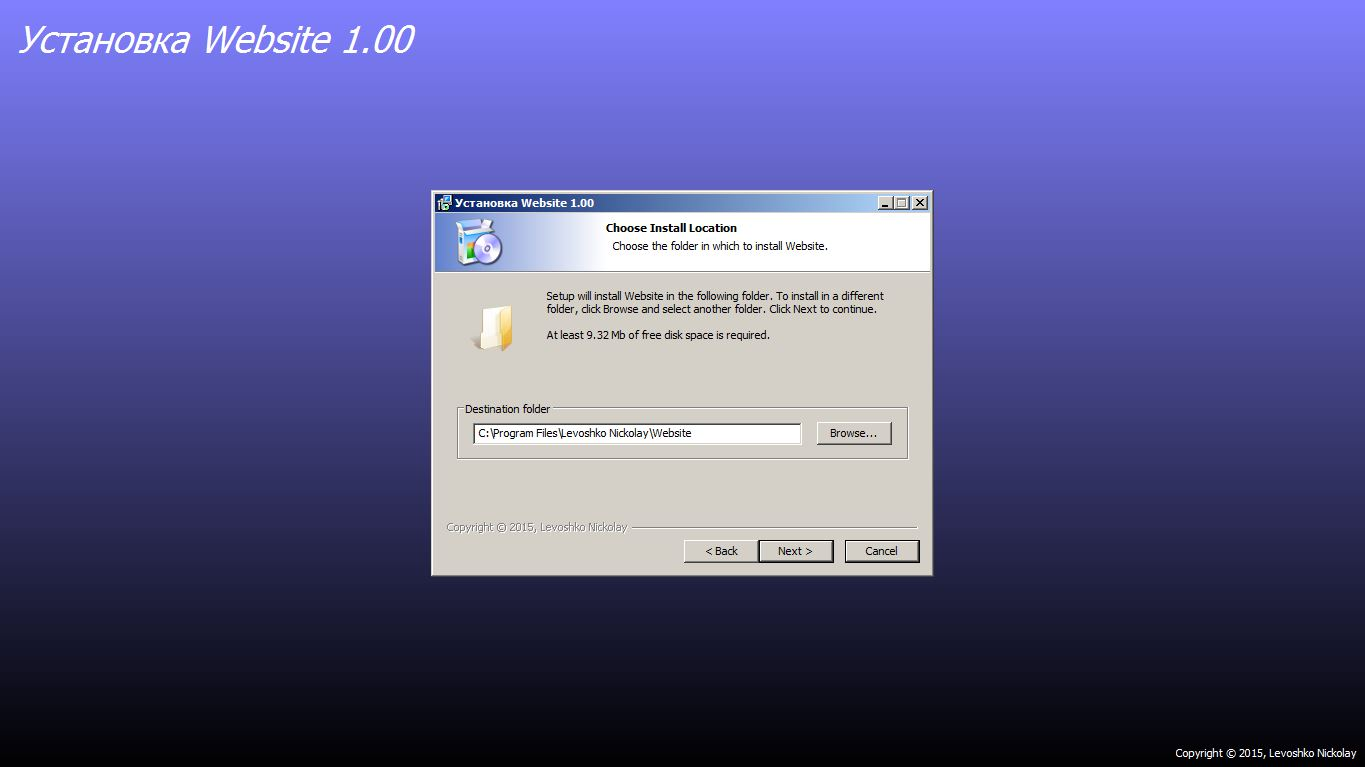
\includegraphics[width=0.7\linewidth]{setuper3}}\\
Третий шаг установки - выбор директории установки.
\center{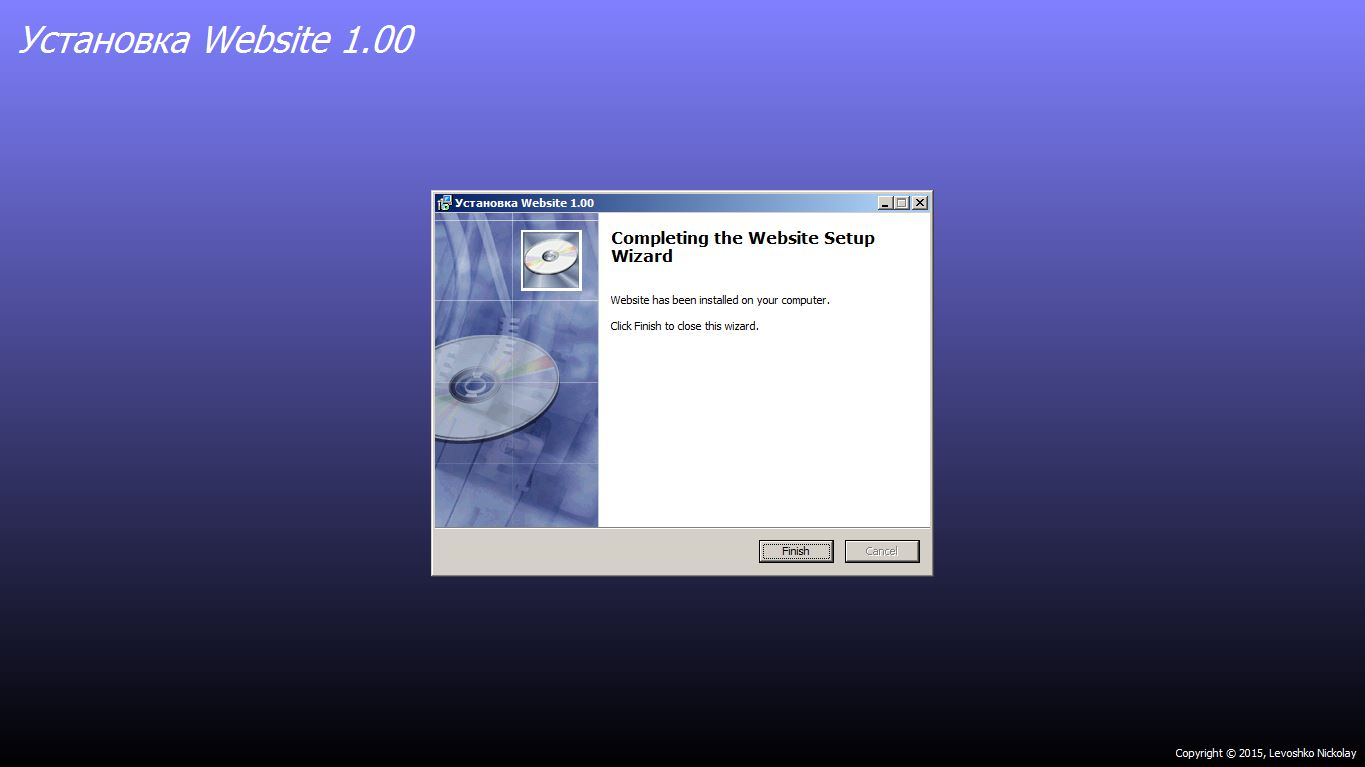
\includegraphics[width=0.7\linewidth]{setuper4}}\\
Последний шаг установки.\\
Приложение готово к использованию.

\newpage
\section*{\normalsize ЗАКЛЮЧЕНИЕ}
\addcontentsline{toc}{section}{ЗАКЛЮЧЕНИЕ}
\hspace{1.25cm}В результате выполнения данного курсового проекта было разработано веб-приложение «Сайт-журнал», позволяющее получать информацию об оказываемых услугах, контактах, были выполнены условиях, требуемые в условии курсового проекта, работает корректно и без сбоев.

На данный момент веб-приложение имеет следующий функционал:

-отображение информации об услугах и их ценах;
-отображение информации о контактах;
-отображение тематических статей;

Работа была разделена на этапы, такие как анализ прототипов,  литературных источников и постановка требований к проектируемому приложению, разработка алгоритма и блок-схемы его работы, конструирование, отладка и тестирование. После последовательного выполнения вышеперечисленных этапов разработки, было получено исправно работающее приложение.

\newpage
\section*{\normalsize СПИСОК ИСПОЛЬЗОВАННОЙ ЛИТЕРАТУРЫ}
\addcontentsline{toc}{section}{СПИСОК ИСПОЛЬЗОВАННОЙ ЛИТЕРАТУРЫ}
	
\hspace{1.25cm}[1] Html and css for real world , Авторы: Alexis Goldstein, Louis Lazaris, Estelle Weyl.

[2] ГОСТ 19.701–90. Единая система программной документации. Схемы алгоритмов, программ, данных и систем. Условные обозначения и правила выполнения. – Введ. 1992–01–01. – М. : Изд-во стандартов, 1991.

[3] JavaScript.ru [Электронный ресурс]. – События : http:/htmlbook.ru.


[4] Habrahabr.ru [Электронный ресурс]. – React : \\
 http://habrahabr.ru/
\newpage
\section*{\normalsize ПРИЛОЖЕНИЕ А(обязательное)}
\addcontentsline{toc}{section}{ПРИЛОЖЕНИЕ А}
\hspace{1.25cm} Код шаблонизатора
\begin{verbatim}
<?php
class Template
{
	private $file;
	
	public function __construct($file)
	{
		$this->file = $file;
	}
	
	public function output()
	{

		$output = file_get_contents($this->file);
			$changed = true;
			while ($changed)
			{
				$changed = false;
				$placeholders = $this->get_placeholders();
				foreach ($placeholders as $key => $value)
				{
					$tag_to_replace = $value;
					$output_copy = $output;
					$template_name = 'templates/' . str_replace("{include(\"", "", $value);
					$template_name = str_replace("\")}", "", $template_name) . '.tpl';
					$output = str_replace($tag_to_replace, file_get_contents($template_name), $output);
					if ($output !== $output_copy)
					{
						$changed = true;
					}
				}
			}		
		return $output;
	}
	
	private function get_placeholders()
	{
		$template = file_get_contents($this->file);
		$pattern = '/{include\(.+?\)}/';
		
		$matches = array();
		preg_match_all($pattern, $template, $matches);
	
		return $matches[0];
	}

	
}	
\end{verbatim}

Код главной страницы
\begin{verbatim}
<?php
include("template.php");
$template = new Template("templates/page-template.html");
echo $template->output();
\end{verbatim}


Код страницы контактов
\begin{verbatim}
<?php
include("template.php");
$template = new Template("templates/page-template-contacts.html");
echo $template->output();
\end{verbatim}


Код страницы цен и услуг
\begin{verbatim}
<?php
include("template.php");
$template = new Template("templates/page-template-price.html");
echo $template->output();
\end{verbatim}


Код страницы статей
\begin{verbatim}
<?php
include("template.php");
$template = new Template("templates/page-template-topics.html");
echo $template->output();
\end{verbatim}


Код html-документа
\begin{verbatim}
<?php
<!DOCTYPE html>
<html >
<head>
    <title>{include("title")}</title>
		<link href="{stylesheet}" rel="stylesheet" />
		<meta http-equiv="content-type" content="text/html; charset=utf-8" />
		<link rel="stylesheet" type="text/css" href="css/index.css" />
		<link rel="stylesheet" type="text/css" href="css/normalize.css"/>   
		<script type="text/javascript" src="js/jquery.js"></script>
		<script type="text/javascript" src="js/easySlider1.7.js"></script>
		<link href="css/screen.css" rel="stylesheet" type="text/css" media="screen" />	
		<script type="text/javascript" src="js/sliderstart.js"></script>
</head>
<body>
    {include("header")}
    {include("content-index")}
	{include("footer")}
</body>
			
</html>

\end{verbatim}

Код footer
\begin{verbatim}
<footer>
	<p><a href="https://vk.com/id220129264"> <img class="icons"  src="img/vk.png" alt="Вконтакте"></a><p>
</footer>
\end{verbatim}



Код header
\begin{verbatim}
<header>
<p><a class="mainlinks" href="index.php">Главная страница</a></p>
</header>
\end{verbatim}


Код содержания главной страницы
\begin{verbatim}
	
			<div id="menu">
			<ul>
			<li><a class="links" href="contacts.php">Контакты</a></li>
			<li><a class="links" href="price.php">Услуги и цены</a></li>
			<li><a class="links" href="topics.php">Статьи</a></li>
			</ul>
			</div>
				<div id="content">
		
					<div id="container">

						<div id="sliderheader">
							<h1>Качественная проводка</h1>
						</div>
							<div id="slidercontent">
								<div id="slider">
									<ul>				
										<li><a href=""><img src="images/03.jpg" alt="Css Template Preview" /></a></li>
										<li><a href=""><img src="images/04.jpg" alt="Css Template Preview" /></a></li>
										<li><a href=""><img src="images/03.jpg" alt="Css Template Preview" /></a></li>
										<li><a href=""><img src="images/04.jpg" alt="Css Template Preview" /></a></li>
										<li><a href=""><img src="images/05.jpg" alt="Css Template Preview" /></a></li>			
									</ul>
								</div>
							</div>

					</div>

				</div>
\end{verbatim}

Код содержания страницы контактов
\begin{verbatim}
			<div id="menu">
			<ul>
			<li><a class="links" href="contacts.php">Контакты</a></li>
			<li><a class="links" href="price.php">Услуги и цены</a></li>
			<li><a class="links" href="topics.php">Статьи</a></li>
			</ul>
			</div>
				<div id="content">content
		
					<div id="container">

						<div id="sliderheader">
							<h1>Качественная проводка</h1>
						</div>
							<div id="slidercontent">
								<div id="slider">
									<ul>				
										<li><a href=""><img src="images/mail.png" alt="mail" /></a></li>
										<li><a href=""><img src="images/phone.png" alt="phone" /></a></li>	
										<li><a href=""><img src="images/adress.png" alt="phone" /></a></li>										
									</ul>
								</div>
							</div>

					</div>

				</div>
\end{verbatim}


Код easyslider
\begin{verbatim}
/*
 * 	Easy Slider 1.7 - jQuery plugin
 *	written by Alen Grakalic	
 *	http://cssglobe.com/post/4004/easy-slider-15-the-easiest-jquery-plugin-for-sliding
 *
 *	Copyright (c) 2009 Alen Grakalic (http://cssglobe.com)
 *	Dual licensed under the MIT (MIT-LICENSE.txt)
 *	and GPL (GPL-LICENSE.txt) licenses.
 *
 *	Built for jQuery library
 *	http://jquery.com
 *
 */
 
/*
 *	markup example for $("#slider").easySlider();
 *	
 * 	<div id="slider">
 *		<ul>
 *			<li><img src="images/01.jpg" alt="" /></li>
 *			<li><img src="images/02.jpg" alt="" /></li>
 *			<li><img src="images/03.jpg" alt="" /></li>
 *			<li><img src="images/04.jpg" alt="" /></li>
 *			<li><img src="images/05.jpg" alt="" /></li>
 *		</ul>
 *	</div>
 *
 */

(function($) {

	$.fn.easySlider = function(options){
	  
		// default configuration properties
		var defaults = {			
			prevId: 		'prevBtn',
			prevText: 		'Previous',
			nextId: 		'nextBtn',	
			nextText: 		'Next',
			controlsShow:	true,
			controlsBefore:	'',
			controlsAfter:	'',	
			controlsFade:	true,
			firstId: 		'firstBtn',
			firstText: 		'First',
			firstShow:		false,
			lastId: 		'lastBtn',	
			lastText: 		'Last',
			lastShow:		false,				
			vertical:		false,
			speed: 			800,
			auto:			false,
			pause:			2000,
			continuous:		false, 
			numeric: 		false,
			numericId: 		'controls'
		}; 
		
		var options = $.extend(defaults, options);  
				
		this.each(function() {  
			var obj = $(this); 				
			var s = $("li", obj).length;
			var w = $("li", obj).width(); 
			var h = $("li", obj).height(); 
			var clickable = true;
			obj.width(w); 
			obj.height(h); 
			obj.css("overflow","hidden");
			var ts = s-1;
			var t = 0;
			$("ul", obj).css('width',s*w);			
			
			if(options.continuous){
				$("ul", obj).prepend($("ul li:last-child", obj).clone().css("margin-left","-"+ w +"px"));
				$("ul", obj).append($("ul li:nth-child(2)", obj).clone());
				$("ul", obj).css('width',(s+1)*w);
			};				
			
			if(!options.vertical) $("li", obj).css('float','left');
								
			if(options.controlsShow){
				var html = options.controlsBefore;				
				if(options.numeric){
					html += '<ol id="'+ options.numericId +'"></ol>';
				} else {
					if(options.firstShow) html += '<span id="'+ options.firstId +'"><a href=\"javascript:void(0);\">'+ options.firstText +'</a></span>';
					html += ' <span id="'+ options.prevId +'"><a href=\"javascript:void(0);\">'+ options.prevText +'</a></span>';
					html += ' <span id="'+ options.nextId +'"><a href=\"javascript:void(0);\">'+ options.nextText +'</a></span>';
					if(options.lastShow) html += ' <span id="'+ options.lastId +'"><a href=\"javascript:void(0);\">'+ options.lastText +'</a></span>';				
				};
				
				html += options.controlsAfter;						
				$(obj).after(html);										
			};
			
			if(options.numeric){									
				for(var i=0;i<s;i++){						
					$(document.createElement("li"))
						.attr('id',options.numericId + (i+1))
						.html('<a rel='+ i +' href=\"javascript:void(0);\">'+ (i+1) +'</a>')
						.appendTo($("#"+ options.numericId))
						.click(function(){							
							animate($("a",$(this)).attr('rel'),true);
						}); 												
				};							
			} else {
				$("a","#"+options.nextId).click(function(){		
					animate("next",true);
				});
				$("a","#"+options.prevId).click(function(){		
					animate("prev",true);				
				});	
				$("a","#"+options.firstId).click(function(){		
					animate("first",true);
				});				
				$("a","#"+options.lastId).click(function(){		
					animate("last",true);				
				});				
			};
			
			function setCurrent(i){
				i = parseInt(i)+1;
				$("li", "#" + options.numericId).removeClass("current");
				$("li#" + options.numericId + i).addClass("current");
			};
			
			function adjust(){
				if(t>ts) t=0;		
				if(t<0) t=ts;	
				if(!options.vertical) {
					$("ul",obj).css("margin-left",(t*w*-1));
				} else {
					$("ul",obj).css("margin-left",(t*h*-1));
				}
				clickable = true;
				if(options.numeric) setCurrent(t);
			};
			
			function animate(dir,clicked){
				if (clickable){
					clickable = false;
					var ot = t;				
					switch(dir){
						case "next":
							t = (ot>=ts) ? (options.continuous ? t+1 : ts) : t+1;						
							break; 
						case "prev":
							t = (t<=0) ? (options.continuous ? t-1 : 0) : t-1;
							break; 
						case "first":
							t = 0;
							break; 
						case "last":
							t = ts;
							break; 
						default:
							t = dir;
							break; 
					};	
					var diff = Math.abs(ot-t);
					var speed = diff*options.speed;						
					if(!options.vertical) {
						p = (t*w*-1);
						$("ul",obj).animate(
							{ marginLeft: p }, 
							{ queue:false, duration:speed, complete:adjust }
						);				
					} else {
						p = (t*h*-1);
						$("ul",obj).animate(
							{ marginTop: p }, 
							{ queue:false, duration:speed, complete:adjust }
						);					
					};
					
					if(!options.continuous && options.controlsFade){					
						if(t==ts){
							$("a","#"+options.nextId).hide();
							$("a","#"+options.lastId).hide();
						} else {
							$("a","#"+options.nextId).show();
							$("a","#"+options.lastId).show();					
						};
						if(t==0){
							$("a","#"+options.prevId).hide();
							$("a","#"+options.firstId).hide();
						} else {
							$("a","#"+options.prevId).show();
							$("a","#"+options.firstId).show();
						};					
					};				
					
					if(clicked) clearTimeout(timeout);
					if(options.auto && dir=="next" && !clicked){;
						timeout = setTimeout(function(){
							animate("next",false);
						},diff*options.speed+options.pause);
					};
			
				};
				
			};
			// init
			var timeout;
			if(options.auto){;
				timeout = setTimeout(function(){
					animate("next",false);
				},options.pause);
			};		
			
			if(options.numeric) setCurrent(0);
		
			if(!options.continuous && options.controlsFade){					
				$("a","#"+options.prevId).hide();
				$("a","#"+options.firstId).hide();				
			};				
			
		});
	  
	};

})(jQuery);




\end{verbatim}


Код запуска слайдера
\begin{verbatim}
$(document).ready(function(){	
			$("#slider").easySlider({
				auto: true, 
				continuous: true
			});
		});	
\end{verbatim}
Код стиля главной страницы
\begin{verbatim}
	@font-face {
 font-family: ariston_normal;
 src: url(ariston_normal.ttf); 
}
header{
font-size: 23pt;
font-style: italic;
text-align: center;
color: black;
font-family: ariston_normal;
}
body {
background-image: url("../img/fonst.jpg");	
background-size: cover;	
}
#menu {
opacity: 0.6;
height:20%;
background-image: url("../img/fonm.jpg");
position: fixed; 	
width: 15%;
color:blue;
border-radius: 40px 10px;
font-size: 15pt;
font-family: ariston_normal;
}
#content {
position:absolute;
margin-left: 15%;
color: black;
height: 100%;
width: 85%;
}
footer {
opacity: 0.6;
background-image: url("../img/fonm.jpg");
position: fixed;
color:white;
bottom: 0;
width: 100%;
height: 11%;
font-size: 15pt;
font-family: ariston_normal;
}
.links {
	text-decoration: none;
	color: aqua;
	}
.mainlinks {
	text-decoration: none;
	color: black;
}
.icons {
width:55px;
height:55px;
margin-left: 0%;
margin-top: 0%;
}
\end{verbatim}

Код стиля слайдера
\begin{verbatim}
	body {
		background:#fff url(../images/bg_body.gif) repeat-x;
		font:80% Trebuchet MS, Arial, Helvetica, Sans-Serif;
		color:#333;
		line-height:180%;
		margin:0;
		padding:0;
		text-align:center;
	}
	h1{
		font-size:180%;
		font-weight:normal;
		margin:0;
		padding:0 20px;
		}
	h2{
		font-size:160%;
		font-weight:normal;
		}	
	h3{
		font-size:140%;
		font-weight:normal;
		}	
	img{border:none;}
	pre{
		display:block;
		font:12px "Courier New", Courier, monospace;
		padding:10px;
		border:1px solid #bae2f0;
		background:#e3f4f9;	
		margin:.5em 0;
		width:674px;
		}	
			
    /* image replacement */
        .graphic, #prevBtn, #nextBtn, #slider1prev, #slider1next{
            margin:0;
            padding:0;
            display:block;
            overflow:hidden;
            text-indent:-8000px;
            }
    /* // image replacement */
			
	#container{	
		margin:0 auto;
		position:relative;
		text-align:left;
		width:696px;
		background:#fff;		
		margin-bottom:2em;
		border: 5px solid #bae2f0;
		}	
	#sliderheader{
		opacity: 0.6;
		height:80px;
		line-height:80px;
		background:#5DC9E1;
		color: White;
		background-image: url("../img/fonm.jpg");
		
		
		}				
	#slidercontent{
		position:relative;
		}			

/* Easy Slider */

	#slider ul, #slider li,
	#slider2 ul, #slider2 li{
		margin:0;
		padding:0;
		list-style:none;
		}
	#slider2{margin-top:1em;}
	#slider li, #slider2 li{ 
		/* 
			define width and height of list item (slide)
			entire slider area will adjust according to the parameters provided here
		*/ 
		width:696px;
		height:241px;
		overflow:hidden; 
		}	
	#prevBtn, #nextBtn,
	#slider1next, #slider1prev{ 
		display:block;
		width:30px;
		height:77px;
		position:absolute;
		left:-30px;
		top:71px;
		z-index:1000;
		}	
	#nextBtn, #slider1next{ 
		left:696px;
		}														
	#prevBtn a, #nextBtn a,
	#slider1next a, #slider1prev a{  
		display:block;
		position:relative;
		width:30px;
		height:77px;
		background:url(../images/btn_prev.gif) no-repeat 0 0;	
		}	
	#nextBtn a, #slider1next a{ 
		background:url(../images/btn_next.gif) no-repeat 0 0;	
		}	
		
	/* numeric controls */	

	ol#controls{
		margin:1em 0;
		padding:0;
		height:28px;	
		}
	ol#controls li{
		margin:0 10px 0 0; 
		padding:0;
		float:left;
		list-style:none;
		height:28px;
		line-height:28px;
		}
	ol#controls li a{
		float:left;
		height:28px;
		line-height:28px;
		border:1px solid #ccc;
		background:#DAF3F8;
		color:#555;
		padding:0 10px;
		text-decoration:none;
		}
	ol#controls li.current a{
		background:#5DC9E1;
		color:#fff;
		}
	ol#controls li a:focus, #prevBtn a:focus, #nextBtn a:focus{outline:none;}
	
/* // Easy Slider */
.sm_slider {
  height: 270px;
  margin: 25px 25px 0px;
  position: relative;
  width: 960px;
}
.sm_slider ul {
  list-style: none;
  margin: 0px;
  padding: 0px;
}

.sm_slide {
  color: #3d3d3d;
  display: none;
  font-size: 100px;
  height: 270px;
  left: 0;
  position: absolute;
  text-align: center;
  top: 0;
  visibility: hidden;
  width: 100%;
}
.sm_slide.active {
  display: block;
  visibility: visible;
}
.sm_slide img {
  max-width: 100%;
}

.sm_prev,
.sm_next {
  width: 25px;
  height: 25px;
  margin: -20px 0 0 0;
  cursor: pointer;
  display: block;
  font-style: normal;
  opacity: .3;
  position: absolute;
  top: 50%;
  z-index: 999;
  border-style: solid;
  border-color: #4e4e4e;
  border-width: 0px;
  -webkit-transform: rotate(-45deg);
  -moz-transform: rotate(-45deg);
  -ms-transform: rotate(-45deg);
  -o-transform: rotate(-45deg);
  transform: rotate(-45deg);
}

.sm_prev {
  border-left-width: 3px;
  border-top-width: 3px;
  left: 10px;
}
.sm_prev:hover {
  opacity: 1;
}

.sm_next {
  border-right-width: 3px;
  border-bottom-width: 3px;
  right: 10px;
}
.sm_next:hover {
  opacity: 1;
}

.sm_nav {
  bottom: 0px;
  clear: both;
  display: inline-block;
  overflow: hidden;
  padding: 5px 0px;
  position: absolute;
  right: 0px;
  z-index: 999;
}

.sm_nav-item {
  cursor: pointer;
  float: left;
  height: 14px;
  padding: 4px;
  width: 14px;
  z-index: 999;
  list-style-type: none;
  font-size: 11px;
  color: #ccc;
}
.sm_nav-item i {
  display: block;
  width: 6px;
  height: 6px;
  position: relative;
  top: 5px;
  left: 4px;
  -webkit-border-radius: 6px;
  -moz-border-radius: 6px;
  -ms-border-radius: 6px;
  -o-border-radius: 6px;
  border-radius: 6px;
  background-color: #7f7f7f;
}
.sm_nav-item.active {
  cursor: default;
  color: #7e7e7e;
}
.sm_nav-item.active:hover {
  cursor: default;
  color: #7e7e7e;
}
.sm_nav-item.active i {
  background-color: #bfbfbf;
}
.sm_nav-item:hover i {
  background: #7f7f7f;
}
.sm_nav-item.active:hover i {
  background-color: #bfbfbf;
}

\end{verbatim}
\end{document}


\end{document}